\documentclass{article}
\usepackage[utf8]{inputenc} % Allow utf-8 input
\usepackage[T1]{fontenc}    % Use 8-bit T1 fonts
\usepackage{graphicx}       % Required for inserting images
\usepackage{booktabs}       % Professional-quality tables
\usepackage{amsfonts}       % Blackboard math symbols
\usepackage{nicefrac}       % Compact symbols for 1/2, etc.
\usepackage{microtype}      % Microtypography
\usepackage[colorlinks=true, linkcolor=blue, citecolor=red, filecolor=magenta, urlcolor=cyan]{hyperref} % Hyperlinks
\usepackage{halloweenmath}
\usepackage{subcaption}
\usepackage{calrsfs}
\usepackage{listings}
\usepackage{authblk}
\usepackage{ragged2e}
\usepackage{amsmath}
\usepackage{amssymb}
\usepackage{color}
\usepackage{amsthm}
\usepackage{bm}
\usepackage{algorithm}
\usepackage{algpseudocode}
\usepackage{dsfont}
\usepackage{bbm}
\usepackage{enumitem}
\usepackage{xcolor}
\usepackage{geometry}
\usepackage{comment}
\usepackage{float}
\usepackage{booktabs}
\usepackage{titling}
\renewcommand\maketitlehooka{\null\mbox{}\vfill}
\renewcommand\maketitlehookd{\vfill\null}

% Define colors for Python syntax highlighting
\definecolor{pythonblue}{RGB}{0,0,255}
\definecolor{pythongreen}{RGB}{0,128,0}
\definecolor{pythonpurple}{RGB}{128,0,128}
\definecolor{pythongray}{RGB}{128,128,128}

\lstdefinelanguage{R}{
    keywords={function, if, else, for, while, repeat, in, next, break},
    keywordstyle=\color{blue}\bfseries,
    ndkeywords={TRUE, FALSE, NULL, Inf, NaN, NA},
    ndkeywordstyle=\color{teal}\bfseries,
    sensitive=true,
    comment=[l]{\#},
    commentstyle=\color{gray}\ttfamily,
    stringstyle=\color{red}\ttfamily,
    morestring=[b]",
    morestring=[b]'
}

\lstset{
    language=R,
    basicstyle=\ttfamily\small,
    showspaces=false,
    showstringspaces=false,
    showtabs=false,
    frame=none, % No box
    tabsize=4,
    captionpos=b,
    breaklines=true,
    breakatwhitespace=true
}

\geometry{a4paper, margin=1in}

\setlength{\parindent}{0pt} % Remove paragraph indentation
\setlength{\parskip}{0.5em} % Add space between paragraphs

\renewcommand{\algorithmicrequire}{\textbf{Input:}}
\renewcommand{\algorithmicensure}{\textbf{Output:}}

\def\c{\boldsymbol{c}}
\def\ud{\underline}
\def\e{\varepsilon}
\def\R{{\mathbb{R}}}
\def\Q{\mathbb{Q}}
\def\Z{\mathcal{Z}}
\def\X{\mathcal{X}}
\def\Y{\mathcal{Y}}
\def\N{\mathbb{N}}
\def\II{{\rm I\kern-0.5exI}}
\def\III{{\rm I\kern-0.5exI\kern-0.5exI}}
\DeclareMathOperator{\grad}{grad}

% == Basic commands == %
\newcommand{\dotprod}[2]{\langle #1, #2 \rangle}
\newcommand{\abs}[1]{\lvert #1 \rvert}
\newcommand{\abss}[1]{\left\lvert #1 \right\rvert}
\newcommand{\norm}[1]{\lVert #1 \rVert}
\newcommand{\normm}[1]{\left\lVert #1 \right\rVert}
\newcommand{\set}[1]{\left\{\, #1 \,\right\}}
\newcommand{\bracket}[1]{\langle #1 \rangle}
\newcommand{\iif}{\Leftrightarrow}
\newcommand{\conv}{\star}

% Sets
\newcommand{\RR}{\mathbb{R}}
\newcommand{\CC}{\mathbb{C}}
\newcommand{\ZZ}{\mathbb{Z}}
\newcommand{\TT}{\mathbb{T}}
\newcommand{\PP}{\mathbb{P}}
\newcommand{\FF}{\mathbb{F}}
\newcommand{\VV}{\mathbb{V}}
\newcommand{\EE}{\mathbb{E}}
\newcommand{\M}{\mathcal{M}}
\newcommand{\Real}{\mathbf{R}}
\newcommand{\Integ}{\mathbf{Z}}
\newcommand{\RN}{\mathbf{R}^N}
\newcommand{\Rd}{\mathbf{R}^d}
\newcommand{\Rn}{\mathbf{R}^n}
\newcommand{\veps}{\varepsilon}
\newcommand{\F}{\mathcal{F}}
\newcommand{\E}{\mathbb{E}}
\newcommand{\I}{\mathcal{I}}
\newcommand{\T}{\mathcal{T}}
\newcommand{\cF}{\mathcal{F}}
\newcommand{\cFall}{\mathcal{F}_{\text{all}}}
\newcommand{\cB}{\mathcal{B}}
\newcommand{\cH}{\mathcal{H}}
\newcommand{\cU}{\mathcal{U}}
\newcommand{\cN}{\mathcal{N}}
\newcommand{\cT}{\mathcal{T}}
\newcommand{\cX}{\mathcal{X}}
\newcommand{\cY}{\mathcal{Y}}
\newcommand{\cZ}{\mathcal{Z}}
\newcommand{\eps}{\varepsilon}
\newcommand{\tx}{\tilde{x}}
\newcommand{\ty}{\tilde{y}}
\newcommand{\tz}{\tilde{z}}
\newcommand{\tA}{\tilde{A}}
\newcommand{\tR}{\tilde{R}}
\newcommand{\tmu}{\tilde{\mu}}
\newcommand{\1}{\mathbbm{1}}
\DeclareMathOperator{\essinf}{essinf}
\DeclareMathOperator{\esssup}{esssup}
\DeclareMathOperator{\supp}{supp}
\DeclareMathOperator{\PRL}{PRL}

% Colors
\newcommand{\red}{\color{red}}
\newcommand{\blue}{\color{blue}}
\newcommand{\nc}{\normalcolor}

\newtheorem{theorem}{Theorem}
\newtheorem{proposition}{Proposition}
\theoremstyle{definition}
\newtheorem{definition}{Definition}
\linespread{1.5}

\makeatletter
\newcommand*\bigcdot{\mathpalette\bigcdot@{.5}}
\newcommand*\bigcdot@[2]{\mathbin{\vcenter{\hbox{\scalebox{#2}{$\m@th#1\bullet$}}}}}
\makeatother

\begin{document}
\title{\textbf{
    Modeling and Forecasting Walmart Stock Prices: A Comparative Analysis of ARMA and GARCH Approaches
}}

\author{Shrivats Sudhir}
\date{December 16, 2023}

\begin{titlingpage}
\maketitle
\end{titlingpage}

\newpage
\tableofcontents
\newpage

\pagenumbering{arabic} % Start normal page numbering
\section{Introduction}

Understanding stock price dynamics is crucial for informed investment decisions. This study models and forecasts Walmart Inc.'s (WMT) daily adjusted closing prices from \texttt{2020-01-01} to \texttt{2023-12-06} with the following objectives: (1) Compute log returns, (2) Find the optimal \texttt{ARIMA} and \texttt{GARCH} models to capture volatility clustering and conditional heteroskedasticity, (3) Fit an ensemble Validate models using AIC, BIC, and residual diagnostics, and (4) Generate a 10-step ahead forecast to provide actionable insights for investors and risk managers by modeling and forecasting stock price movements.

Let $P_t$ be the price of an asset at time $t$, then the log returns is defined as:
$$r_t = \text{log}\;P_t - \text{log}\;P_{t-1}$$

The code for computing log returns and bollinger bands can be found \hyperref[subsec:loading_data]{here}. 

\begin{figure}[H]
\centering
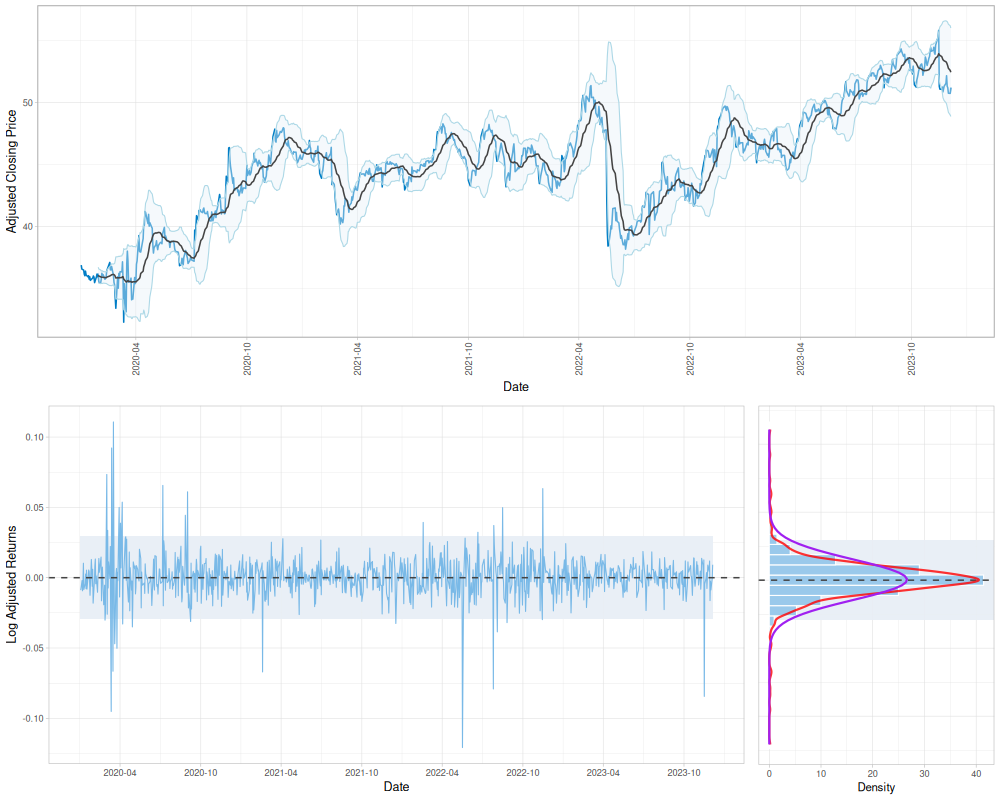
\includegraphics[width=1.0\textwidth]{Walmart_Stock_Analysis.png}
\caption{\small{\hyperref[subsec:adjclose_adjreturns_plot]{Walmart Inc.'s adjusted closing prices with Bollinger Bands, log returns with a 95\% confidence interval, and a histogram of log returns with KDE and theoretical normal distribution.}}}
\label{fig:adjclose_adjreturns_plot}
\end{figure}

From \hyperref[fig:adjclose_adjreturns_plot]{Figure \ref{fig:adjclose_adjreturns_plot}}, there seems to exist some volatility clusters that need to be addressed. Furthermore, the log return distribution seems to be Leptokurtic in nature, illustrating heavy tails and deviations from normality. We now proceed with rigorously testing for normality and stationarity.








\section{Fitting \texttt{ARIMA} Model}

The \texttt{forecast} package in R allows us to use \texttt{auto.arima} which automatically selects the best model based on AIC/BIC.

\begin{table}[H]
\centering
\begin{tabular}{l|r}
\hline
\textbf{Model}  & \textbf{ARIMA(0,0,1) with zero mean} \\
\hline
MA1 Coefficient & -0.0666 \\
Standard Error  & 0.0312 \\
$\sigma^2$      & 0.0002266 \\
\hline
Log-Likelihood  & 2694.43 \\
AIC             & -5384.85 \\
AICc            & -5384.84 \\
BIC             & -5375.1 \\
\hline
\end{tabular}
\caption{\small{\hyperref[subsec:arma_model_summary]{Summary of fitted ARMA model.}}}
\label{tab:arma_model_summary}
\end{table}

The fitted \texttt{ARIMA(0,0,1)} model for Walmart Inc.'s log returns is summarized in \hyperref[tab:arma_model_summary]{Table \ref{tab:arma_model_summary}}, with a moving average coefficient of $-0.0666$ (standard error = $0.0312$), indicating weak short-term autocorrelation. The residual variance is estimated as $\sigma^2 = 0.0002266$, and model selection criteria, including AIC ($-5384.85$) and BIC ($-5375.1$), confirm its suitability.

In mathematical terms, we can write the \texttt{ARIMA} model as:
$$r_t = a_t - (-0.0666) \cdot a_{t-1}$$
where $a_t \sim N(0, 0.0312)$ and $\mathbb{E}[r_t] = 0$.


\section{Fitting \texttt{ARCH/GARCH} Models}

The \texttt{fGarch} library in R allows us to fit various \texttt{GARCH} models and compare performances between the them. For the purposes of keeping the models simple and explainable, the focus is on \texttt{GARCH}(1,0) and \texttt{GARCH}(1,1), using conditional distributions from \texttt{c("norm", "ged", "std", "snorm", "sged", "sstd")}.

\begin{table}[H]
\centering
\begin{minipage}[t]{0.48\textwidth} % Left table (Normality Tests)
\centering
\scriptsize % Reduce font size
\begin{tabular}{l|r}
\hline
\textbf{Model}  & \texttt{GARCH(1,0), cond.dist="std"} \\
\hline
mu & 6.090e-04\\
omega & 1.505e-04\\
alpha1 & 2.988e-01\\
shape & 3.436e+00\\
\hline
Log-Likelihood  & 2908.097 \\
AIC             & -5.987829 \\
BIC             & -5.967716 \\
SIC             & -5.987863\\
HQIC            & -5.980173\\
\hline
\end{tabular}
\end{minipage}
\hfill
\begin{minipage}[t]{0.48\textwidth} % Right table (Stationarity Tests)
\centering
\scriptsize % Reduce font size
\begin{tabular}{l|r}
\hline
\textbf{Model}  & \texttt{GARCH(1,1), cond.dist="std"} \\
\hline
mu              & 5.220e-04\\
omega           & 1.560e-05\\
alpha1          & 1.291e-01\\
beta1           & 7.905e-01\\
shape           & 4.062e+00\\
\hline
Log-Likelihood  & 2929.534 \\
AIC             & -6.029967 \\
BIC             & -6.004826 \\
SIC             & -6.030020\\
HQIC            & -6.020398\\
\hline
\end{tabular}
\end{minipage}
\caption{\small{\hyperref[subsec:arch_garch_model_summary]{Summary of fitted \texttt{GARCH(1,0)} and \texttt{GARCH(1,1)} model, with students-t conditional distribution.}}}
\label{tab:arch_garch_model_summary}
\end{table}

\hyperref[tab:arch_garch_model_summary]{Table \ref{tab:arch_garch_model_summary}} summarizes the fitted \texttt{GARCH(1,0)} and \texttt{GARCH(1,1)} models using a Student-t conditional distribution, which among all other conditional distribution options best maximizes log-likelihood with reasonable AIC, BIC, SIC, HQIC values. Although \texttt{GARCH(1,0)} achieves slightly lower AIC (-5.99 vs. -6.03) and BIC (-5.97 vs. -6.00), indicating a marginally better balance between model fit and complexity, we find that \texttt{GARCH(1,1)} achieves a higher log-likelihood (2929.534 vs. 2908.097) and captures long-term volatility persistence through the additional $\beta_1$ parameter, which is crucial for financial time series exhibiting volatility clustering. Therefore, we prefer \texttt{GARCH(1,1)} over \texttt{GARCH(1,0)}.

In mathematical terms, we can write the \texttt{GARCH(1,1)} model as:
$$a_t = \sigma_t \epsilon_t, \quad \sigma^2_t = (\text{1.560e-05}) + (\text{1.291e-01})a^2_{t-1} + (\text{7.905e-01})\sigma^2_{t-1}$$
where $\epsilon_t \sim \text{std}(0,1)$ with shape parameter 4.0624. The relatively large value of $\beta_1$ (0.7905) relative to $\alpha_1$ (0.1291) reflects the long memory in volatility, which is consistent with financial time series exhibiting volatility clustering.






\section{Fitting Ensemble $\texttt{ARIMA(0,0,1)}+\texttt{GARCH(1,1)}$ Model}

A preliminary $\texttt{ARIMA(0,0,1)}+\texttt{GARCH(1,1)}$ model with a Student-t conditional distribution is fitted to the log returns to capture volatility clustering and heavy tails. We iteratively detect and remove influential points (standardized residuals exceeding a threshold of $\pm 3$) by fitting until the process continues until no new influential points are identified, or the changes in residual diagnostics become negligible.

\begin{table}[H]
\centering
\begin{tabular}{l|r}
\hline
\textbf{Model}  & \texttt{ARIMA(0,0,1) + GARCH(1,1)} \\
\hline
mu & 4.9198e-04 \\
omega  & 6.3505e-06 \\
alpha1      & 1.0224e-01 \\
beta1 & 8.5001e-01\\
shape & 1.0000e+01\\
\hline
Log-Likelihood  & 2972.232\\
AIC             & -6.246803\\
BIC             & -6.221243\\
SIC             & -6.246858\\
HQIC            & -6.237065\\
\hline
\end{tabular}
\caption{\small{\hyperref[subsec:arma_garch_model_summary]{Summary of fitted \texttt{ARMA(0,0,1)+GARCH(1,1)} model.}}}
\label{tab:arma_garch_model_summary}
\end{table}

From \hyperref[tab:arma_garch_model_summary]{Table \ref{tab:arma_garch_model_summary}}, we can see that there is a substantial increase in log-likelihood compared to individual \texttt{GARCH(1,1)} or \texttt{ARIMA(0,0,1)} models, with only slight increase in AIC and BIC. Furthermore, the statistically significant $\beta_1$ value (0.8501) indicates strong long-term persistence in volatility, while the moderate statistically significant $\alpha_1$ value (0.1022) captures short-term shocks effectively.








\section{Residual Diagnostics}

\hyperref[fig:residual_diagnostics]{Figure \ref{fig:residual_diagnostics}} show that the fitted ensemble model is satisfactory. The residuals over time are random around zero, the histogram aligns with a normal distribution, the Q-Q plot shows minimal deviation from normality, and the ACF plots confirm no significant autocorrelation in residuals, squared residuals, or absolute residuals, indicating no remaining structure or volatility clustering.

\begin{figure}[H]
\centering
\begin{subfigure}{\textwidth}
    \centering
    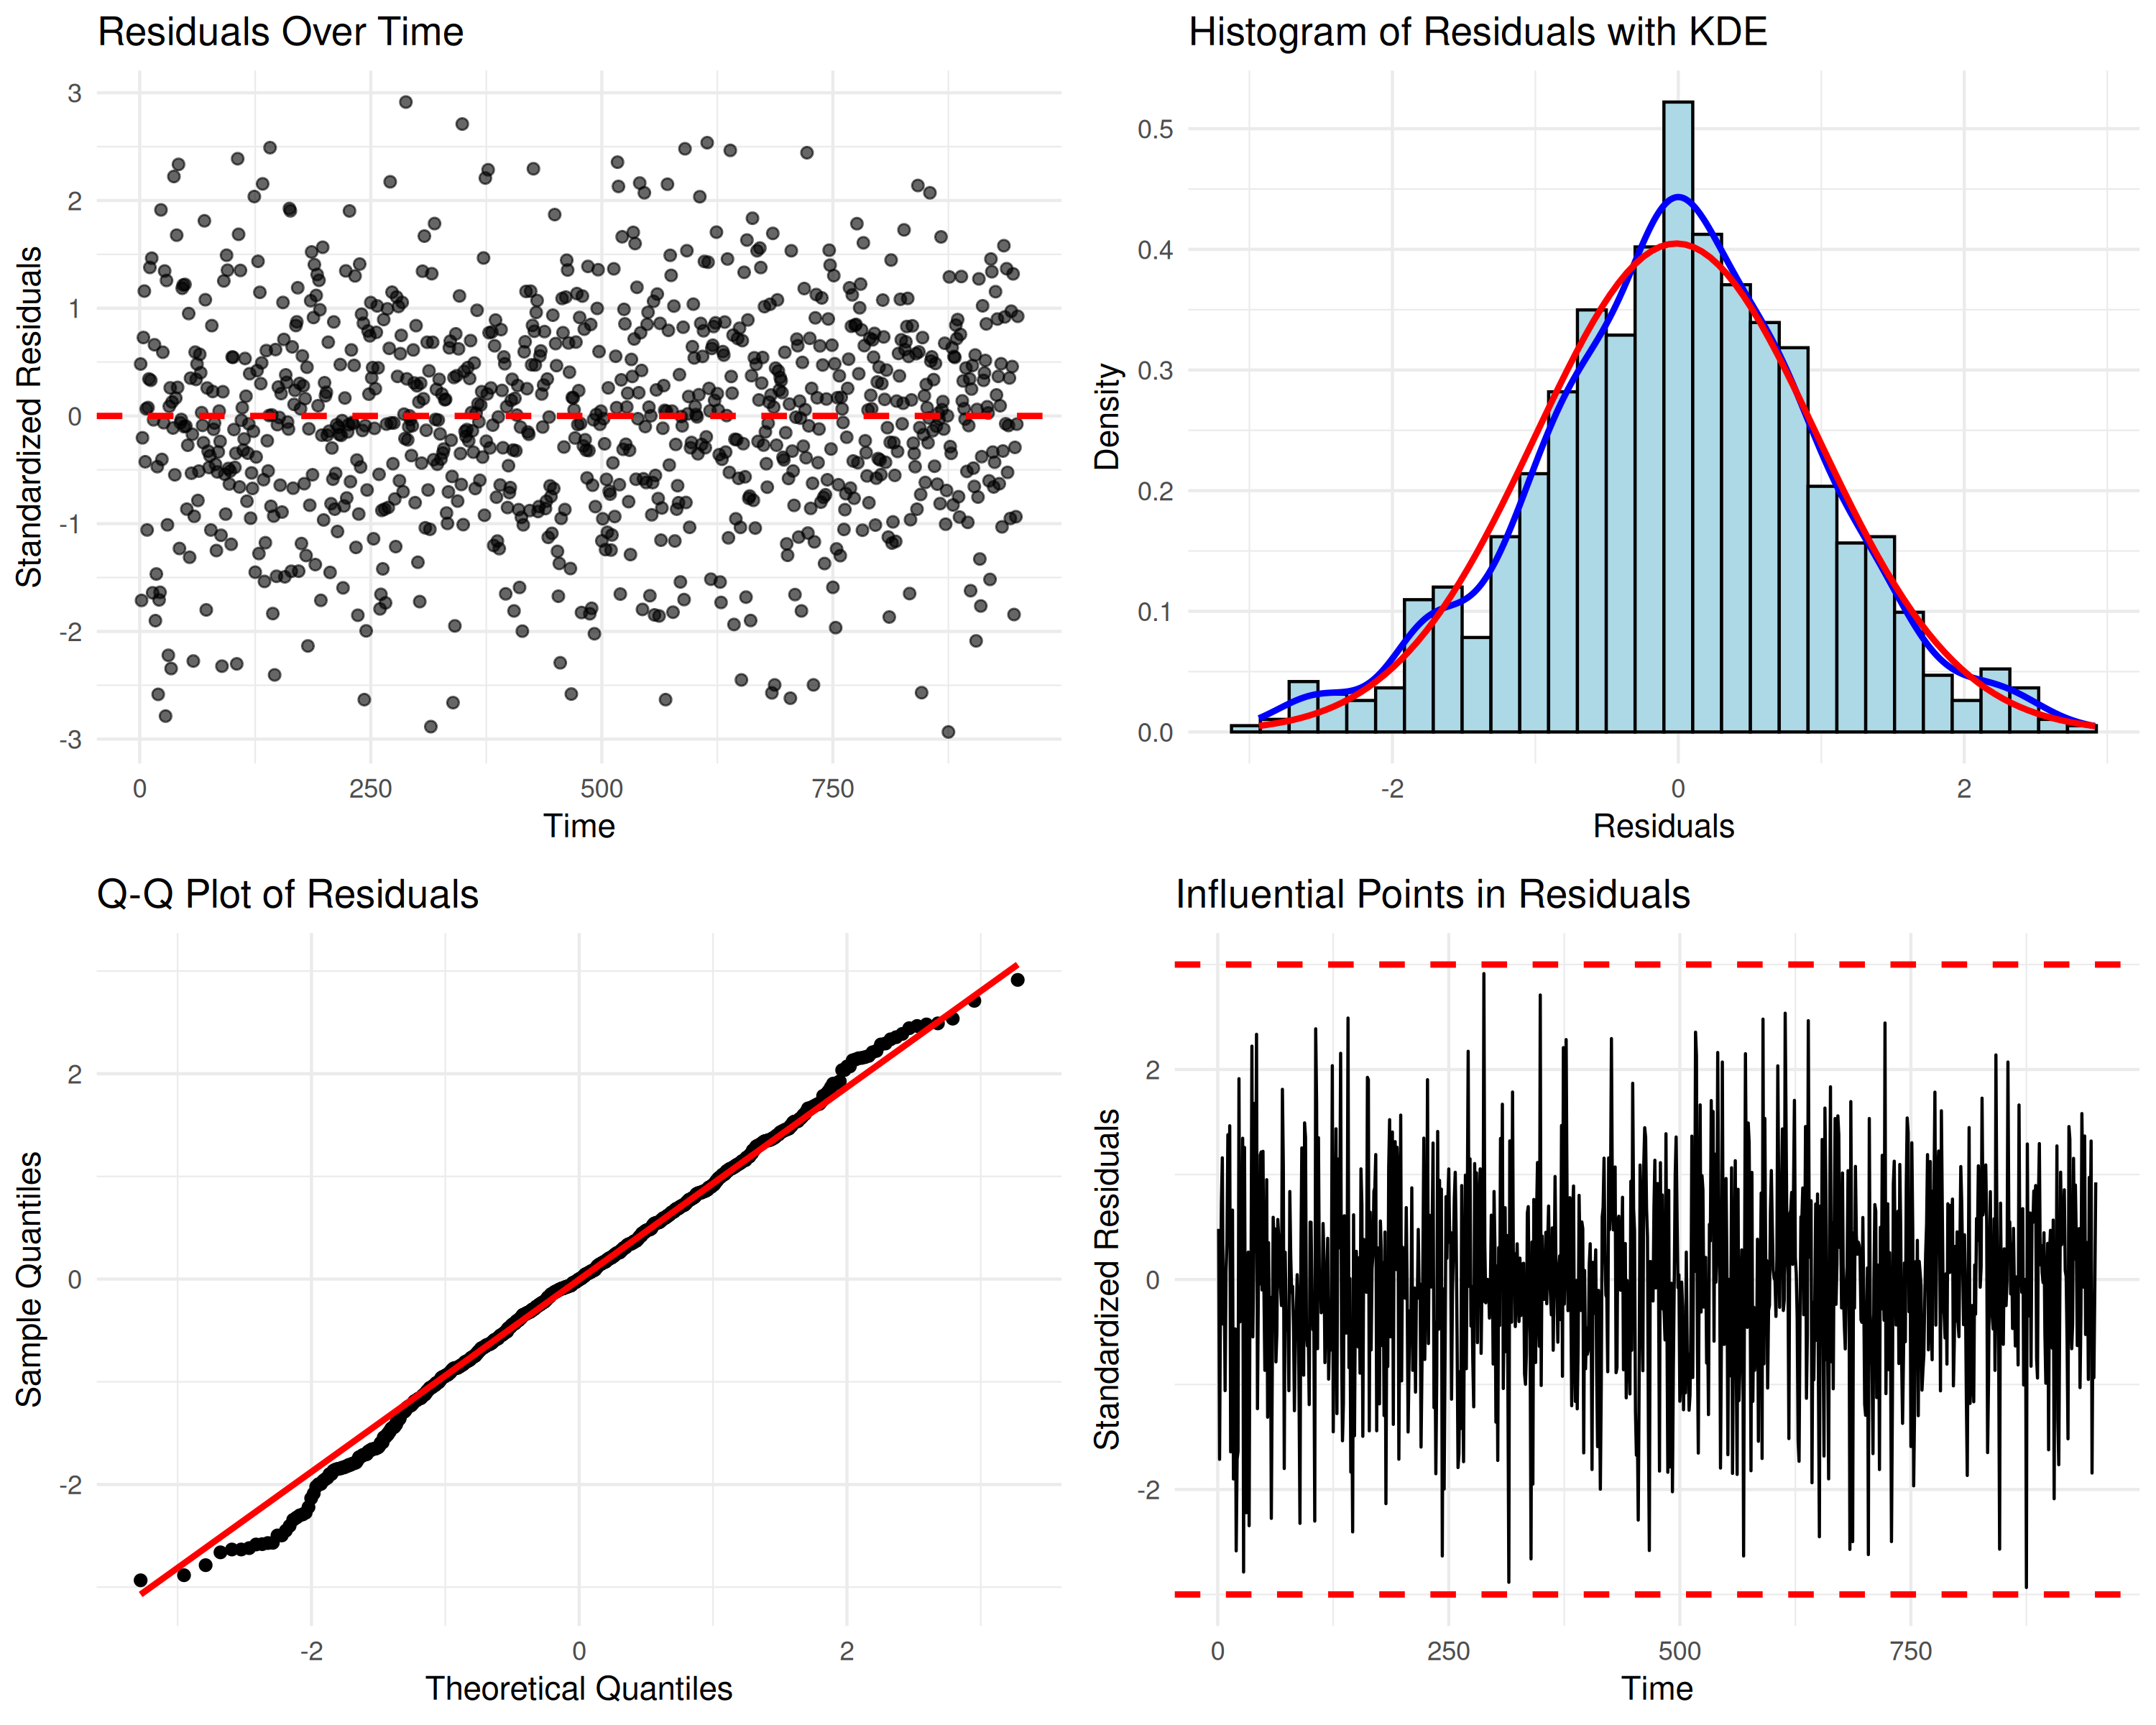
\includegraphics[width=0.8\textwidth]{Residual_Diagnostics.png}
\end{subfigure}

\begin{subfigure}{\textwidth}
    \centering
    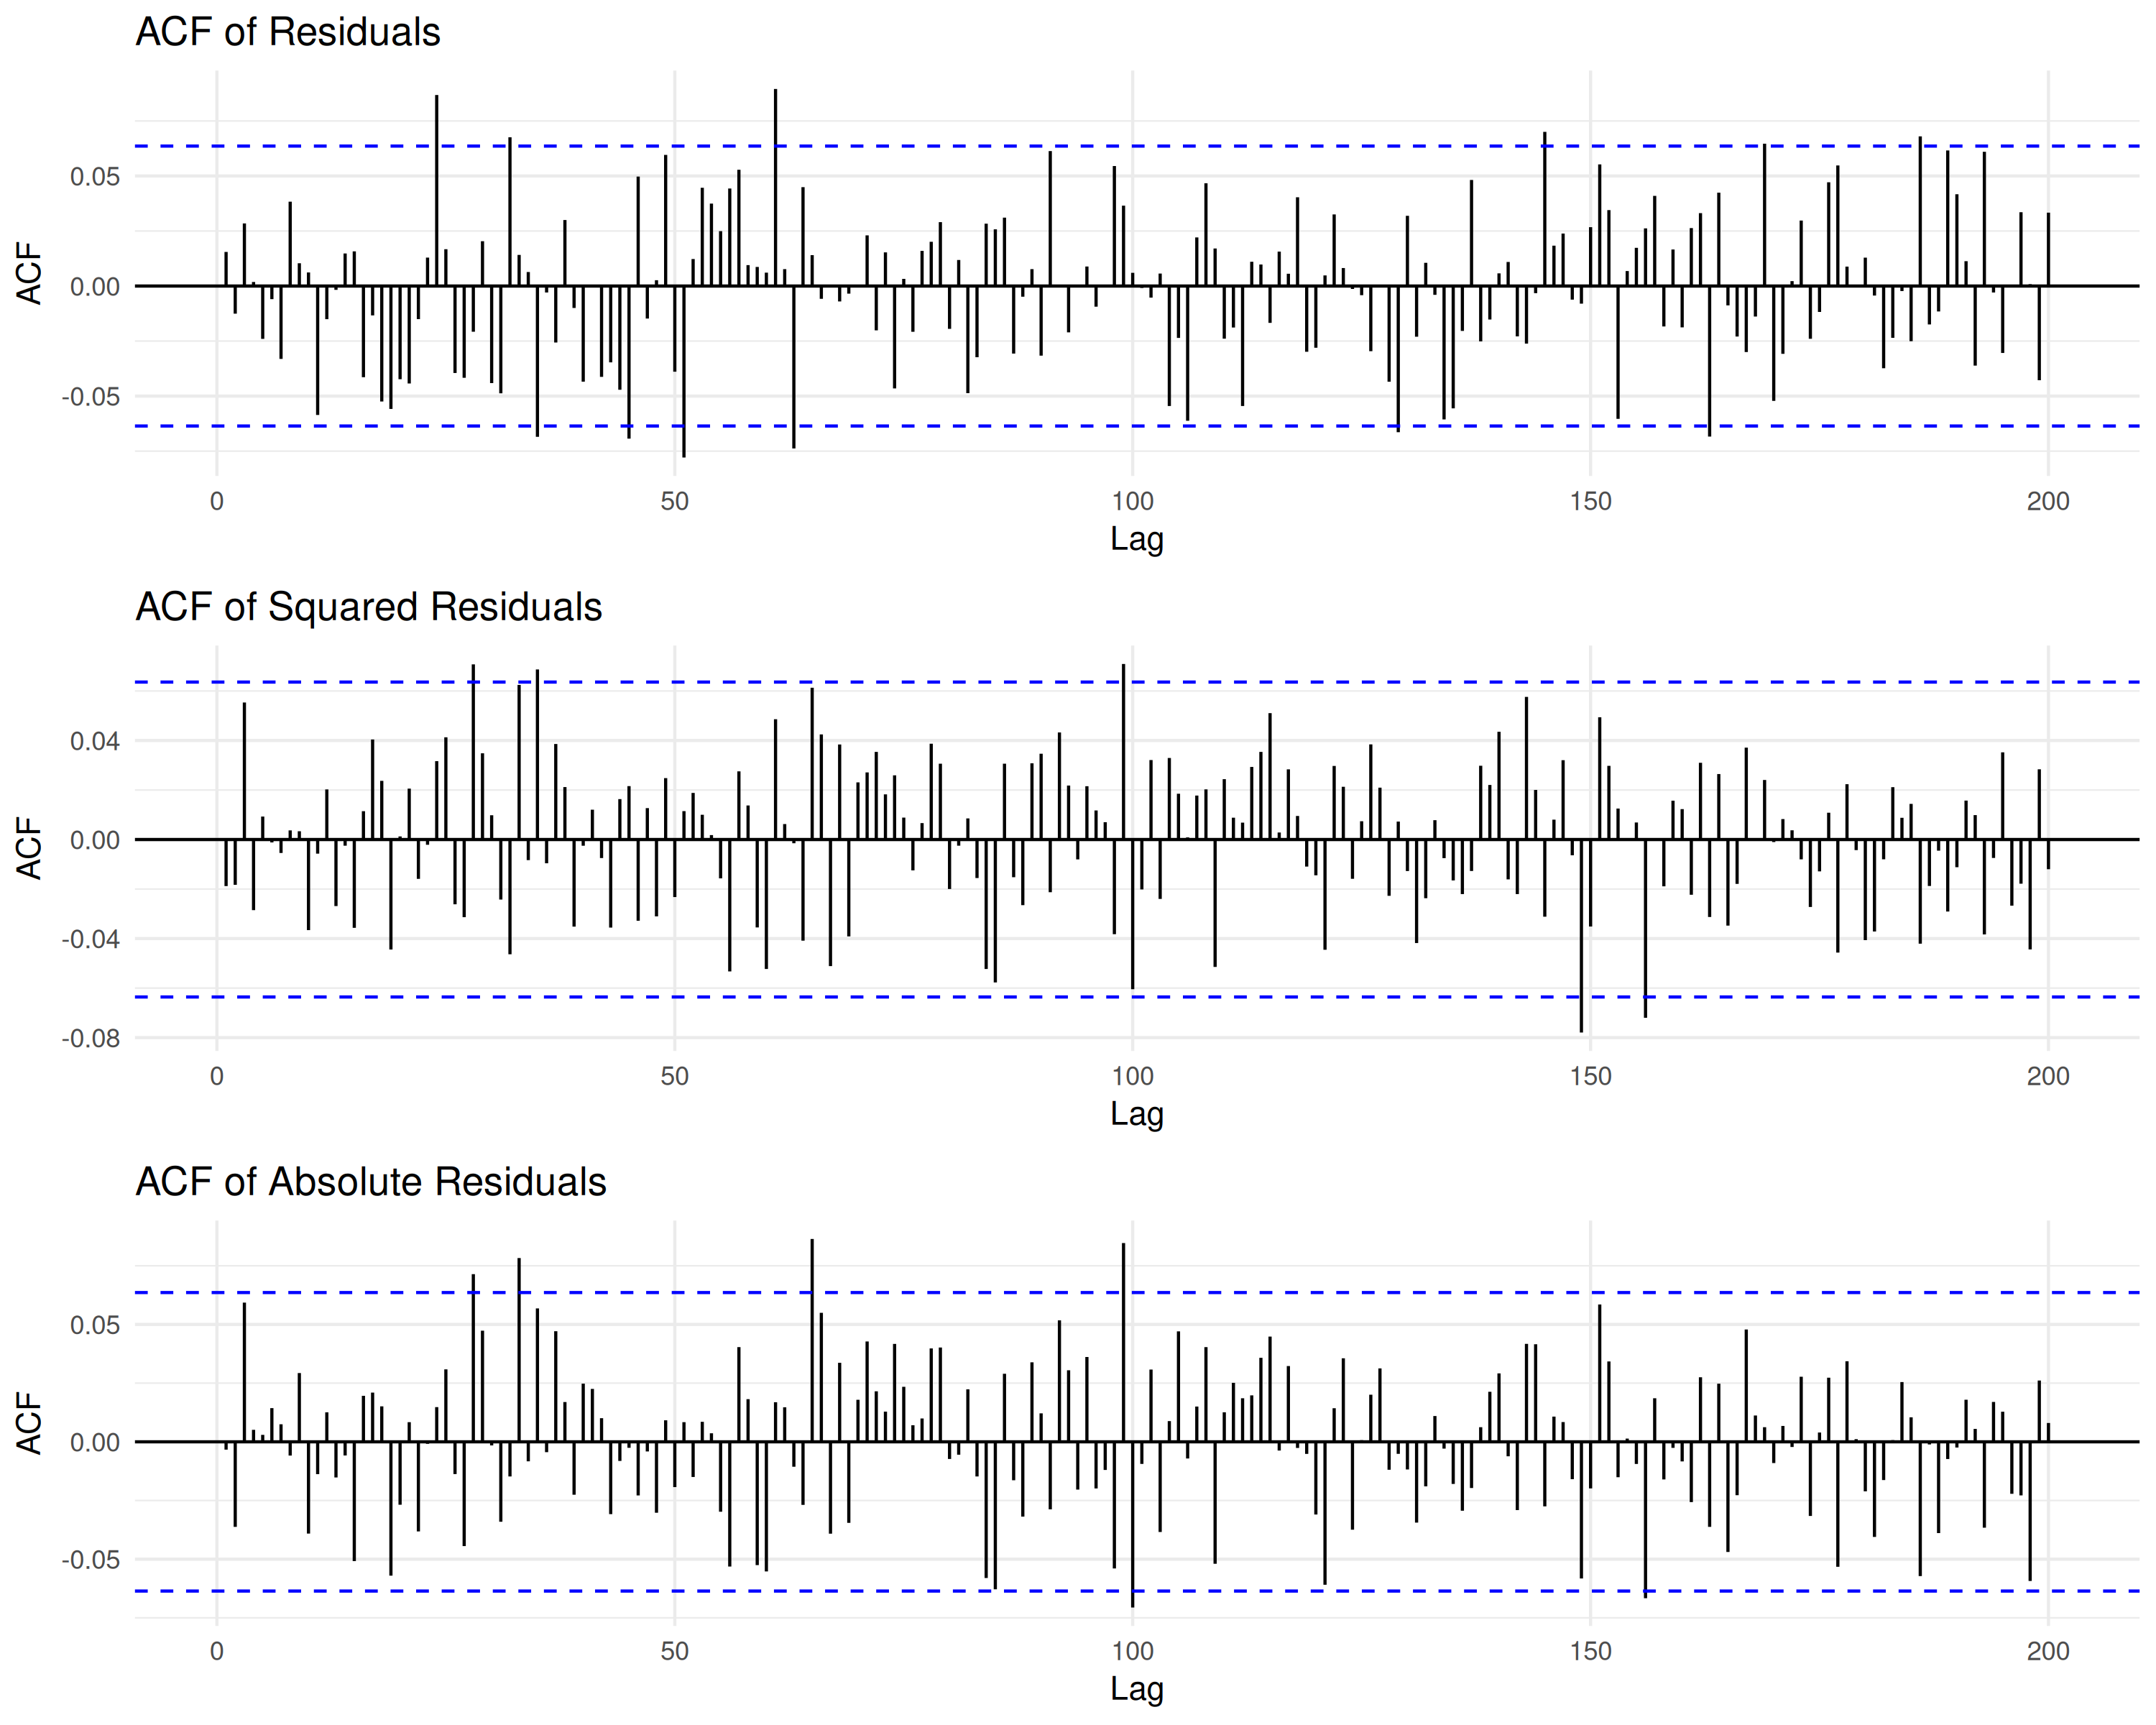
\includegraphics[width=0.75\textwidth]{ACF_plots.png}
\end{subfigure}

\caption{\small{\hyperref[subsec:residual_diagnostics]{Residual diagnostics for the $\texttt{ARIMA(0,0,1)} + \texttt{GARCH(1,1)}$ model.}}}
\label{fig:residual_diagnostics}
\end{figure}










\section{10-Day Forecast}

\begin{figure}[H]
\centering
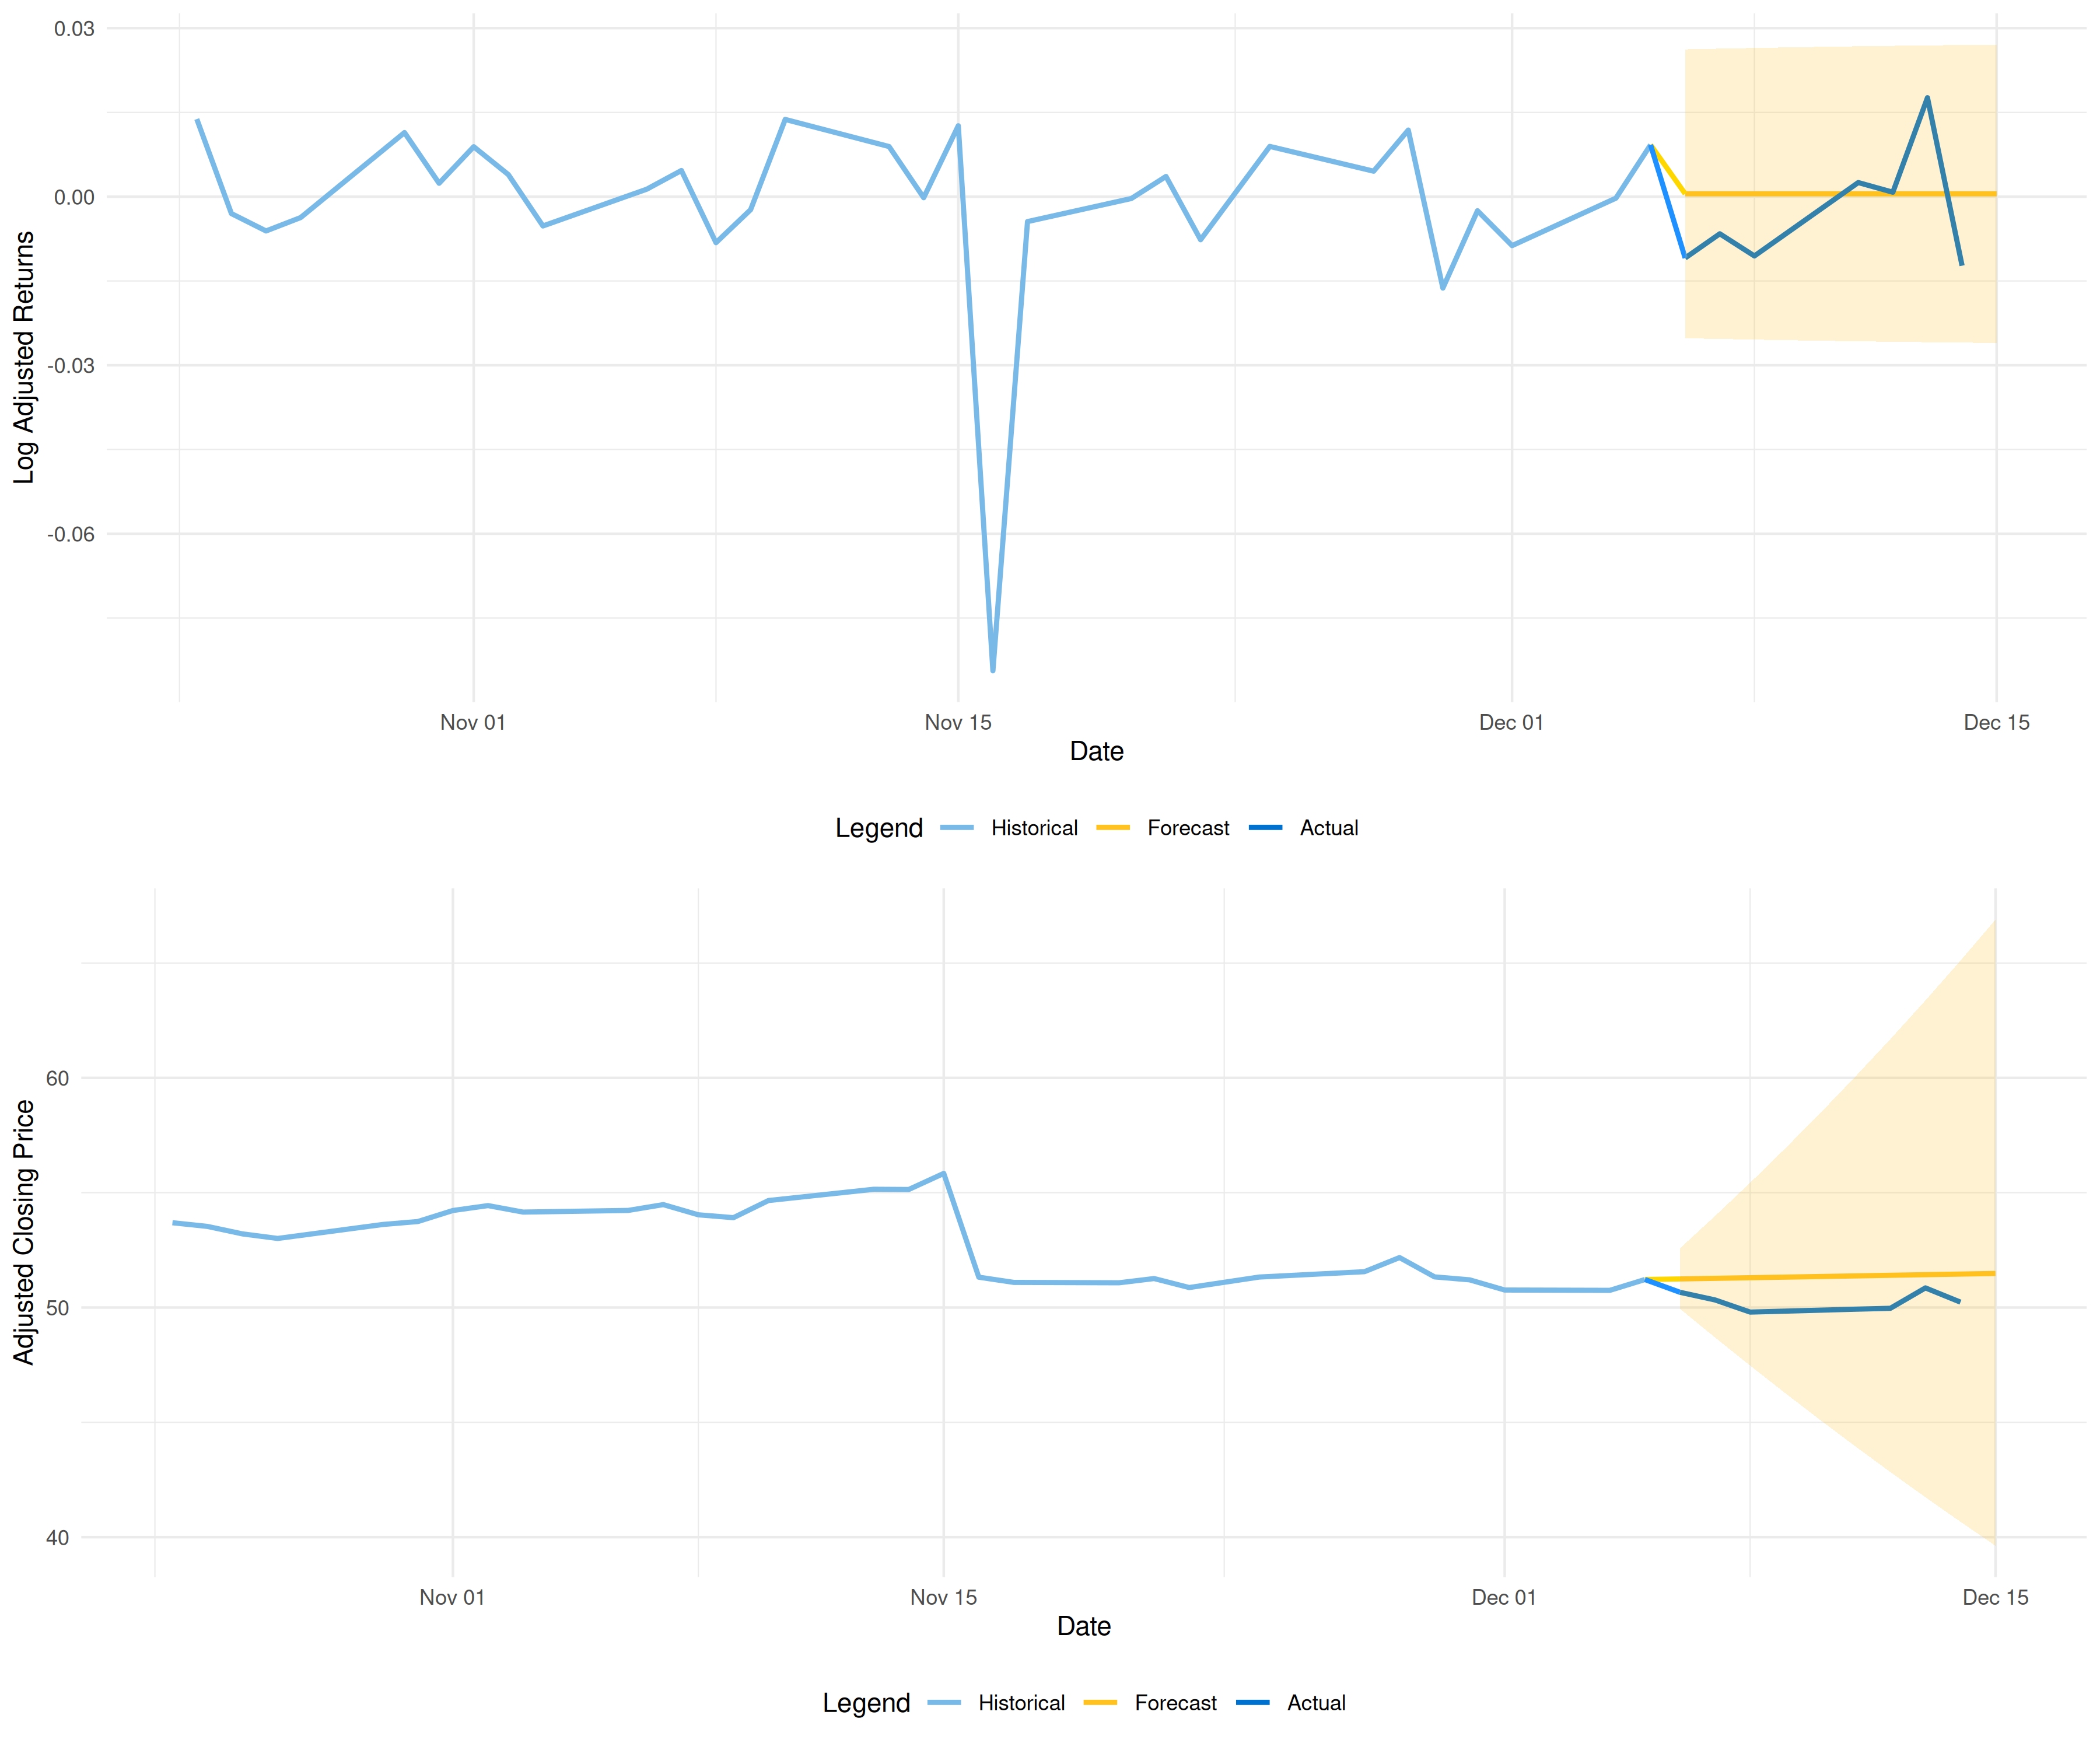
\includegraphics[width=1.0\textwidth]{Forecast.png}
\caption{\small{\hyperref[subsec:forecast]{10-day forecast for log returns and adjusted closing prices, including 95\% confidence intervals, alongside historical and actual data for comparison. (last 30+10 days only). Blue represents historical data, yellow indicates the forecast, and dark blue corresponds to actual observed values.}}}
\label{fig:forecast}
\end{figure}

\hyperref[fig:forecast]{Figure \ref{fig:forecast}} allows us to compare our 10-day forecast with the true log returns and adjusted closing price. It is crucial to note that the model only fits data from \texttt{2020-01-01} to \texttt{2023-12-05}. The actual log returns from \texttt{2023-12-06} to \texttt{2023-12-15} is used to compare model performance on unseen data.

The forecasted log returns align well with the actual values, with all observations falling within the 95\% confidence interval. This indicates that the $\texttt{ARIMA(0,0,1)} + \texttt{GARCH(1,1)}$ model effectively captures the short-term dynamics of the stock. However, the increasing width of the confidence interval for closing prices reflects the compounding effect of forecast uncertainty over time. The RMSE for the 10-day forecast, actual log returns, and adjusted prices were \$ 0.0103 and \$ 1.1693, respectively.

Given the residual diagnostics in \hyperref[fig:residual_diagnostics]{Figure \ref{fig:residual_diagnostics}} affirmation that the $\texttt{ARIMA(0,0,1)} + \texttt{GARCH(1,1)}$ model effectively captures the underlying structure of Walmart's stock returns, we can conclude that this is a good and effective model for forecasting.



\newpage
\section{Reference}

Bollerslev, T. (1986). Generalized autoregressive conditional heteroskedasticity. Journal of Econometrics, 31(3), 307-327. \url{https://doi.org/10.1016/0304-4076(86)90063-1}.\\

Box, George E. P., et al. Time Series Analysis: Forecasting and Control. United Kingdom, Wiley, 2008. \url{https://www.google.com/books/edition/Time_Series_Analysis/lJnnPQAACAAJ?hl=en}.\\

Campbell, John Y., et al. The Econometrics of Financial Markets. Princeton University Press, 1997. JSTOR, \url{https://doi.org/10.2307/j.ctt7skm5}.\\

Engle, Robert F. Autoregressive Conditional Heteroscedasticity with Estimates of the Variance of United Kingdom Inflation. Econometrica, vol. 50, no. 4, 1982, pp. 987–1007. JSTOR, \url{https://doi.org/10.2307/1912773}.\\

Hansen, P. R., \& Lunde, A. (2005). A forecast comparison of volatility models: Does anything beat a GARCH(1,1)? Journal of Applied Econometrics, 20(7), 873-889. \url{https://doi.org/10.1002/jae.800}.\\

Pfaff, Bernhard. (2008). Analysis of Integrated and Cointegrated Time Series with R. DOI: \url{https://doi.org/10.1007/978-0-387-75967-8}.\\

Poon, Ser-Huang, and Clive W.J. Granger. 2003. Forecasting Volatility in Financial Markets: A Review. Journal of Economic Literature, 41 (2): 478–539. DOI: \url{https://doi.org/10.1257/002205103765762743}.




\newpage
\section{Appendix}

\subsection{Code for R Library Imports}
\label{subsec:library_imports}

\begin{lstlisting}[language=R]
rm(list = ls())

# Install required libraries
if (!require("quantmod")) install.packages("quantmod", dependencies = TRUE)
if (!require("fBasics")) install.packages("fBasics", dependencies = TRUE)
if (!require("fGarch")) install.packages("fGarch", dependencies = TRUE)
if (!require("timeSeries")) install.packages("timeSeries", dependencies = TRUE)
if (!require("zoo")) install.packages("zoo", dependencies = TRUE)
if (!require("reactable")) install.packages("reactable", dependencies = TRUE)
if (!require("ggplot2")) install.packages("ggplot2", dependencies = TRUE)
if (!require("grid")) install.packages("grid", dependencies = TRUE)
if (!require("gridExtra")) install.packages("gridExtra", dependencies = TRUE)
if (!require("tseries")) install.packages("tseries", dependencies = TRUE)
if (!require("forecast")) install.packages("forecast", dependencies = TRUE)
if (!require("dplyr")) install.packages("dplyr", dependencies = TRUE)

library(quantmod)
library(fBasics)
library(fGarch)
library(timeSeries)
library(zoo)
library(reactable)
library(ggplot2)
library(grid)
library(gridExtra)
library(tseries)
library(forecast)
library(dplyr)
\end{lstlisting}

\subsection{Code for Loading Data:}
\label{subsec:loading_data}

\begin{lstlisting}[language=R]
getSymbols("WMT", from = "2020-01-01", to = "2023-12-06") 
AdjClose = Ad(WMT) # Adjusted Close Prices

# Create a data frame with adjusted close prices and log returns
WMT_df <- data.frame(
  Date = index(AdjClose),
  AdjClose = coredata(AdjClose),
  LogReturns = c(NA, diff(log(coredata(AdjClose))))
)

# Rename columns for clarity
colnames(WMT_df) <- c("Date", "AdjClose", "LogReturns")

# Load csv
WMT_df <- read.csv("Walmart_AdjPrice.csv")
WMT_df$Date <- as.Date(WMT_df$Date, format = "%Y-%m-%d")

# Calculate Bollinger Bands
rolling_mean <- rollmean(WMT_df$AdjClose, k = 20, fill = NA, align = "right")
rolling_sd <- rollapply(WMT_df$AdjClose, width = 20, FUN = sd, 
                        fill = NA, align = "right")
bollinger_upper <- rolling_mean + 2 * rolling_sd
bollinger_lower <- rolling_mean - 2 * rolling_sd

# Add Bollinger Bands to the data frame
WMT_df$BollingerMean <- rolling_mean
WMT_df$BollingerUpper <- bollinger_upper
WMT_df$BollingerLower <- bollinger_lower

WMT_df <- na.omit(WMT_df)
\end{lstlisting}


\subsection{Code for Figure \ref{fig:adjclose_adjreturns_plot}:}
\label{subsec:adjclose_adjreturns_plot}

\begin{lstlisting}[language=R]
# Compute empirical statistics for Walmart's log returns
empirical_mean <- mean(WMT_df$LogReturns, na.rm = TRUE)
empirical_sd <- sd(WMT_df$LogReturns, na.rm = TRUE)
ci_lower <- empirical_mean - 1.96 * empirical_sd
ci_upper <- empirical_mean + 1.96 * empirical_sd

# Normal distribution for comparison
normal_x <- seq(min(WMT_df$LogReturns,
                    na.rm = TRUE), 
                max(WMT_df$LogReturns, 
                    na.rm = TRUE), length.out = 100)
normal_y <- dnorm(normal_x, mean = empirical_mean, sd = empirical_sd)

# Plot 1: Adjusted Close Prices with Bollinger Bands
price_plot <- ggplot(WMT_df, aes(x = Date)) +
  geom_line(aes(y = AdjClose), linewidth = 0.7, 
            na.rm = TRUE, color = "#007dc6") +
  geom_ribbon(aes(ymin = BollingerLower, ymax = BollingerUpper), 
              alpha = 0.4, fill = "#e7f0f7", na.rm = TRUE) +
  geom_line(aes(y = BollingerUpper), linetype = "solid", 
            linewidth = 0.5, na.rm = TRUE, color = "lightblue") +
  geom_line(aes(y = BollingerLower), linetype = "solid", 
            linewidth = 0.5, na.rm = TRUE, color = "lightblue") +
  geom_line(aes(y = BollingerMean), 
            linewidth = 0.7, na.rm = TRUE, color = "#444444") +
  theme_light() +
  labs(x = "Date", y = "Adjusted Closing Price") +
  scale_x_date(date_breaks = "6 months", date_labels = "%Y-%m") +
  theme(
    axis.text.x = element_text(angle = 90, vjust = 0.5, hjust = 1),
    plot.title = element_text(size = 14, face = "bold"),
    axis.title = element_text(size = 12),
    legend.position = "none" # Remove legend
  )

# Plot 2: Time-Series of Log Returns
time_series_plot <- ggplot(WMT_df, aes(x = Date)) +
  geom_rect(aes(xmin = min(Date, na.rm = TRUE), 
                xmax = max(Date, na.rm = TRUE), 
                ymin = ci_lower, 
                ymax = ci_upper), alpha = 0.3, fill = "#e7f0f7") +
  geom_line(aes(y = LogReturns), 
            linewidth = 0.5, na.rm = TRUE, color = "#79b9e7") +
  geom_hline(yintercept = 0.0, 
             color = "#444", linetype = "dashed", linewidth = 0.7) +
  theme_light() +
  labs(x = "Date", y = "Log Adjusted Returns") +
  scale_x_date(date_breaks = "6 months", date_labels = "%Y-%m") +
  theme(
    legend.position = "none", # Remove legend
    axis.title = element_text(size = 12)
  )

# Plot 3: Rotated Histogram of Log Returns
rotated_histogram <- ggplot(WMT_df, aes(x = LogReturns)) +
  geom_rect(aes(xmin = ci_lower, xmax = ci_upper), 
            ymin = 0, ymax = Inf, alpha = 0.3, fill = "#e7f0f7") +
  geom_histogram(aes(y = after_stat(density)), 
                 binwidth = 0.0075, color = "white", 
                 alpha = 0.7, fill = "#79b9e7", na.rm = TRUE) +
  geom_vline(xintercept = 0.0, color = "#444", 
             linetype = "dashed", linewidth = 0.7) +
  stat_density(geom = "line", color = "red", 
               linewidth = 1, alpha = 0.8, na.rm = TRUE) +
  geom_line(data = data.frame(x = normal_x, y = normal_y), 
            aes(x = x, y = y), color = "purple", linewidth = 1) +
  coord_flip() +
  labs(x = "", y = "Density") +
  theme_light() +
  theme(
    legend.position = "none", # Remove legend
    axis.text.y = element_blank(),
    axis.ticks.y = element_blank(),
    axis.title.y = element_blank()
  )

# Combine bottom row
bottom_row <- arrangeGrob(grobs = list(time_series_plot, rotated_histogram),
                          ncol = 2, widths = c(3, 1))

# Arrange the final layout
final_layout <- grid.arrange(
  price_plot,       # Top row
  bottom_row,       # Bottom two plots
  nrow = 2,         # Two rows
  heights = c(1, 1) # Adjust row heights
)
\end{lstlisting}

\subsection{Code for Table \ref{tab:arma_model_summary}:}
\label{subsec:arma_model_summary}

\begin{lstlisting}
# Fit best ARMA model automatically
arma_fit <- auto.arima(WMT_df$LogReturns, seasonal = FALSE)
print(summary(arma_fit))
\end{lstlisting}

\subsection{Code for Table \ref{tab:arch_garch_model_summary}:}
\label{subsec:arch_garch_model_summary}

\begin{lstlisting}
# Fit ARCH / GARCH(1,0)
fit_arch <- garchFit(~ garch(1, 0), data = WMT_df$LogReturns, cond.dist = "std")
summary(fit_arch)

# Fit GARCH(1,1)
fit_garch <- garchFit(~ garch(1, 1), data = WMT_df$LogReturns, cond.dist = "std")
summary(fit_garch)
\end{lstlisting}

\subsection{Code for Table \ref{tab:arma_garch_model_summary}:}
\label{subsec:arma_garch_model_summary}

\begin{lstlisting}
# Initialize cleaned data
data_cleaned <- WMT_df$LogReturns

# Threshold for influential points (standardized residuals)
threshold <- 3

# Iterative process to remove influential points
iteration <- 1
repeat {
  cat("\nIteration:", iteration, "\n")
  
  # Fit ARMA+GARCH(1,1) model
  arma_garch_model <- garchFit(~arma(0,0,1) + garch(1,1), 
                               data = data_cleaned, 
                               cond.dist = "std", 
                               trace = FALSE)
  
  # Extract standardized residuals
  residuals_model <- residuals(arma_garch_model, standardize = TRUE)
  
  # Identify influential points
  influential_points <- which(abs(residuals_model) > threshold)
  cat("Number of influential points detected:", length(influential_points), "\n")
  
  # Stop if no more influential points are found
  if (length(influential_points) == 0) {
    cat("No more influential points. Stopping iteration.\n")
    break
  }
  
  # Remove influential points and refit
  data_cleaned <- data_cleaned[-influential_points]
  cat("Removed influential points at indices:", influential_points, "\n")
  
  iteration <- iteration + 1
}

# Final model with cleaned data
arma_garch_model <- garchFit(~arma(0,0,1) + garch(1,1), 
                                     data = data_cleaned, 
                                     cond.dist = "std", 
                                     trace = FALSE)

# Model summary
print(summary(arma_garch_model))
\end{lstlisting}


\subsection{Code for Figure \ref{fig:residual_diagnostics}}
\label{subsec:residual_diagnostics}

\begin{lstlisting}[language=R]
# Extract standardized residuals for the cleaned model
residuals_cleaned <- residuals(arma_garch_model, standardize=TRUE)

# 1. Residuals over time
residuals_time <- data.frame(Time=1:length(residuals_cleaned), 
                             Residuals=residuals_cleaned)
p1 <- ggplot(residuals_time, aes(x=Time, y=Residuals)) +
  geom_point(alpha=0.6) +
  geom_hline(yintercept=0, color="red", linetype="dashed", linewidth=1) +
  labs(title="Residuals Over Time", x="Time", y="Standardized Residuals") +
  theme_minimal()

# 2. Residual histogram with KDE and theoretical distribution
p2 <- ggplot(data.frame(Residuals = residuals_cleaned), aes(x = Residuals)) +
  geom_histogram(aes(y = after_stat(density)), 
                 bins=30, fill="lightblue", color="black") +
  geom_density(color = "blue", linetype = "solid", linewidth=1) +
  stat_function(fun=dnorm, args=list(mean=mean(residuals_cleaned), 
                                     sd=sd(residuals_cleaned)), 
                color="red", linetype="solid", linewidth=1) +
  labs(title = "Histogram of Residuals with KDE", x = "Residuals", y = "Density") +
  theme_minimal()

# Q-Q Plot of residuals
p3 <- ggplot(data.frame(Residuals = residuals_cleaned), aes(sample = Residuals)) +
  stat_qq() +
  stat_qq_line(color = "red", linewidth=1) +
  labs(title = "Q-Q Plot of Residuals", x = "Theoretical Quantiles", y = "Sample Quantiles") +
  theme_minimal()

# Influential points graph (standardized residuals > 3 or < -3)
influential_points_cleaned <- which(abs(residuals_cleaned) > 3)
influential_residuals <- residuals_time[influential_points_cleaned, ]

p4 <- ggplot(residuals_time, aes(x = Time, y = Residuals)) +
  geom_line() +
  geom_hline(yintercept = c(-3, 3), color = "red", 
             linetype = "dashed", linewidth=1) +
  labs(title = "Influential Points in Residuals", x = "Time", y = "Standardized Residuals") +
  theme_minimal()

# Display the plots
residual_plots <- grid.arrange(p1, p2, 
                               p3, p4, ncol=2, nrow=2)

# ACF plots (Residuals, Squared Residuals, Absolute Residuals)
acf_residuals_plot <- ggAcf(residuals_cleaned, lag.max=200) +
  ggtitle("ACF of Residuals") +
  theme_minimal()

# ACF of squared residuals
acf_squared_residuals_plot <- ggAcf(residuals_cleaned^2, lag.max=200) +
  ggtitle("ACF of Squared Residuals") +
  theme_minimal()

# ACF of absolute residuals
acf_abs_residuals_plot <- ggAcf(abs(residuals_cleaned), lag.max=200) +
  ggtitle("ACF of Absolute Residuals") +
  theme_minimal()

# Display the plots
ACF_plots <- grid.arrange(acf_residuals_plot, 
                          acf_squared_residuals_plot, 
                          acf_abs_residuals_plot, ncol = 1)
\end{lstlisting}


\subsection{Code for Figure \ref{fig:forecast}:}
\label{subsec:forecast}

\begin{lstlisting}[language=R]
# Forecast parameters
forecast_length <- 10
last_date <- max(WMT_df$Date)
last_price <- tail(WMT_df$AdjClose, 1)
last_log_return <- tail(WMT_df$LogReturns, 1)

# Forecast log returns
forecasts <- predict(arma_garch_model, n.ahead = forecast_length, plot = FALSE)

# Create forecast dataframe
forecast_df <- data.frame(
  Date = seq(last_date + 1, by = 1, length.out = forecast_length),
  LogReturns = forecasts$meanForecast,
  Lower95 = forecasts$meanForecast - 1.96 * forecasts$standardDeviation,
  Upper95 = forecasts$meanForecast + 1.96 * forecasts$standardDeviation
)

# Calculate prices and confidence intervals
forecast_df$AdjPrice <- last_price * exp(cumsum(forecast_df$LogReturns))
forecast_df$LowerAdjPrice <- last_price * exp(cumsum(forecast_df$Lower95))
forecast_df$UpperAdjPrice <- last_price * exp(cumsum(forecast_df$Upper95))

# Fetch actual recent prices
getSymbols("WMT", from = last_date, 
           to = last_date + forecast_length, 
           auto.assign = TRUE)

# Prepare actual prices dataframe
actual_prices <- data.frame(
  Date = index(WMT),
  AdjClose = as.numeric(Ad(WMT))
)
actual_prices$LogReturns <- c(NA, diff(log(actual_prices$AdjClose)))
actual_prices <- na.omit(actual_prices)

# Prepare recent historical data
recent_historical_data <- tail(WMT_df, 30)

# Prepare connecting lines for price
connect_price <- data.frame(
  Date = c(last_date, forecast_df$Date[1], last_date, actual_prices$Date[1]),
  AdjClose = c(last_price, forecast_df$AdjPrice[1], 
               last_price, actual_prices$AdjClose[1]),
  Connector = c("Forecast Connector", "Forecast Connector", 
                "Historical Connector", "Historical Connector")
)

# Prepare connecting lines for log returns
connect_log_returns <- data.frame(
  Date = c(last_date, forecast_df$Date[1], last_date, actual_prices$Date[1]),
  LogReturns = c(last_log_return, forecast_df$LogReturns[1], 
                 last_log_return, actual_prices$LogReturns[1]),
  Connector = c("Forecast Connector", "Forecast Connector", 
                "Historical Connector", "Historical Connector")
)

# Convert to date
connect_price$Date <- as.Date(connect_price$Date)
connect_log_returns$Date <- as.Date(connect_log_returns$Date)

palette <- c(
  "Historical" = "#79b9e7",
  "Forecast" = "#FFC220",
  "Actual" = "#0071CE",
  "Forecast Connector" = "#FFD700",  # Yellow
  "Historical Connector" = "#1E90FF" # Blue
)
# Price Plot
price_plot <- ggplot() +
  # Historical price line
  geom_line(data = recent_historical_data, 
            aes(x = Date, y = AdjClose, color = "Historical"), size = 1) +
  # Forecast price line
  geom_line(data = forecast_df, 
            aes(x = Date, y = AdjPrice, color = "Forecast"), size = 1) +
  # Actual market prices line
  geom_line(data = actual_prices, 
            aes(x = Date, y = AdjClose, color = "Actual"), size = 1) +
  # Connecting lines (with legend suppressed)
  geom_line(data = connect_price, 
            aes(x = Date, y = AdjClose, color = Connector, linetype = Connector), 
            size = 1, show.legend = FALSE) +
  # Confidence interval ribbon
  geom_ribbon(data = forecast_df, 
              aes(x = Date, ymin = LowerAdjPrice, ymax = UpperAdjPrice), 
              fill = "#FFC220", alpha = 0.2) +
  scale_color_manual(values = palette,
                     name = "Legend",
                     breaks = c("Historical", "Forecast", "Actual")) +
  scale_linetype_manual(values = c("Forecast Connector" = "solid", 
                                   "Historical Connector" = "solid")) +
  labs(
    x = "Date",
    y = "Adjusted Closing Price"
  ) +
  theme_minimal() +
  theme(
    plot.title = element_text(hjust = 0.5, face = "bold"),
    legend.position = "bottom",
  )

# Log Returns Plot
log_return_plot <- ggplot() +
  # Historical log returns
  geom_line(data = recent_historical_data, 
            aes(x = Date, y = LogReturns, color = "Historical"), size = 1) +
  # Forecast log returns
  geom_line(data = forecast_df, 
            aes(x = Date, y = LogReturns, color = "Forecast"), size = 1) +
  # Actual market log returns
  geom_line(data = actual_prices, 
            aes(x = Date, y = LogReturns, color = "Actual"), size = 1) +
  # Connecting lines (with legend suppressed)
  geom_line(data = connect_log_returns, 
            aes(x = Date, y = LogReturns, color = Connector, linetype = Connector), 
            size = 1, show.legend = FALSE) +
  # Confidence interval ribbon
  geom_ribbon(data = forecast_df, 
              aes(x = Date, ymin = Lower95, ymax = Upper95), 
              fill = "#FFC220", alpha = 0.2) +
  scale_color_manual(values = palette,
                     name = "Legend",
                     breaks = c("Historical", "Forecast", "Actual")) +
  scale_linetype_manual(values = c("Forecast Connector" = "solid", 
                                   "Historical Connector" = "solid")) +
  labs(
    x = "Date",
    y = "Log Adjusted Returns"
  ) +
  theme_minimal() +
  theme(
    plot.title = element_text(hjust = 0.5, face = "bold"),
    legend.position = "bottom",
  )

# Combine and save plots
forecast_plot <- grid.arrange(log_return_plot, price_plot, ncol = 1)

# Align forecast_df and actual_prices by Date
aligned_data <- inner_join(forecast_df, actual_prices, by = "Date", suffix = c("_forecast", "_actual"))

# Calculate RMSE for log returns
log_returns_rmse <- sqrt(mean((aligned_data$LogReturns_forecast - aligned_data$LogReturns_actual)^2, na.rm = TRUE))
cat("RMSE for Log Returns: ", log_returns_rmse, "\n")

# Calculate RMSE for adjusted prices
price_rmse <- sqrt(mean((aligned_data$AdjPrice - aligned_data$AdjClose)^2, na.rm = TRUE))
cat("RMSE for Adjusted Prices: ", price_rmse, "\n")
\end{lstlisting}


\newpage
\subsection{Public GitHub Repository}
All codes and images associated with this project can be found in the GitHub repository below:

\begin{center}
\url{https://github.com/Stochastic1017/Walmart-Stock-Forecasting}
\end{center}

\textit{Note: The repository will be made public after \textbf{December 18, 2024 (00:00 AM)} to ensure academic integrity by preventing public access to these materials before the due date.}\\

\begin{table}[H]
\centering
\begin{tabular}{l|r}
\hline
\textbf{Figure/Table}  & \textbf{Code} \\
\hline
Figure \ref{fig:adjclose_adjreturns_plot} & \href{https://github.com/Stochastic1017/Walmart-Stock-Forecasting/blob/main/R/Plot_AdjClose_LogReturns.R}{Code for Figure \ref{fig:adjclose_adjreturns_plot}} \\
Table \ref{tab:arma_model_summary} & \href{https://github.com/Stochastic1017/Walmart-Stock-Forecasting/blob/main/R/Fit_ARMA.R}{Code for Table \ref{tab:arma_model_summary}} \\
Table \ref{tab:arch_garch_model_summary} & \href{https://github.com/Stochastic1017/Walmart-Stock-Forecasting/blob/main/R/Fit_ARCH_GARCH.R}{Code for Table \ref{tab:arch_garch_model_summary}} \\
Table \ref{tab:arma_garch_model_summary} & \href{https://github.com/Stochastic1017/Walmart-Stock-Forecasting/blob/main/R/Fit_ARMA_and_GARCH.R}{Code for Table \ref{tab:arma_garch_model_summary}} \\
Figure \ref{fig:residual_diagnostics} & \href{https://github.com/Stochastic1017/Walmart-Stock-Forecasting/blob/main/R/Plot_Residual_Diagnostics.R}{Code for Figure \ref{fig:residual_diagnostics}} \\
Figure \ref{fig:forecast} & \href{https://github.com/Stochastic1017/Walmart-Stock-Forecasting/blob/main/R/Plot_Forecast.R}{Code for Figure \ref{fig:forecast}} \\
\hline
\end{tabular}
\end{table}

For a more comprehensive analysis and consolidated access to all the code used in the manner in which it was intended, the following files are available in the repository. Note that these greatly exceeds the 5-page limit and consolidates all R codes and outputs used for this project:

\begin{table}[H]
\centering
\begin{tabular}{l|r}
\hline
\textbf{File}  & \textbf{URL} \\
\hline
\texttt{Consolidated-Walmart-Stock-Forecasting.Rmd} & \href{https://github.com/Stochastic1017/Walmart-Stock-Forecasting/blob/main/Rmd/Walmart-Stock-Forecasting.Rmd}{Rmd File Link} \\
\texttt{Consolidated-Walmart-Stock-Forecasting.pdf} & \href{https://github.com/Stochastic1017/Walmart-Stock-Forecasting/blob/main/Rmd/Walmart-Stock-Forecasting.pdf}{PDF File Link} \\
\hline
\end{tabular}
\end{table}

Finally, the LaTeX file and the rendered pdf file associated to this submission write-up is available in this repository:

\begin{table}[H]
\centering
\begin{tabular}{l|r}
\hline
\textbf{File}  & \textbf{URL} \\
\hline
\texttt{Walmart-Stock-Forecasting.tex} & \href{https://github.com/Stochastic1017/Walmart-Stock-Forecasting/blob/main/Write-Up/Walmart-Stock-Forecasting.tex}{TEX File Link} \\
\texttt{Walmart-Stock-Forecasting.pdf} & \href{https://github.com/Stochastic1017/Walmart-Stock-Forecasting/blob/main/Write-Up/Walmart_Stock_Forecasting.pdf}{PDF File Link} \\
\hline
\end{tabular}
\end{table}


\end{document}
